
\begin{figure}
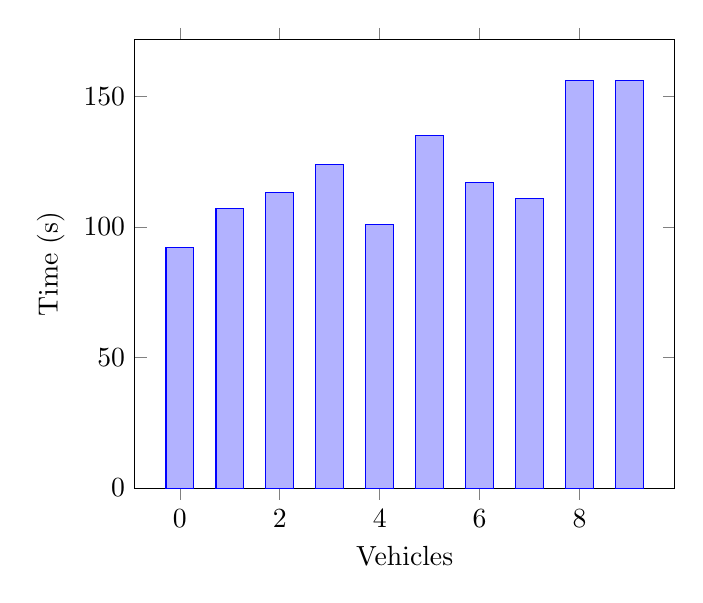
\begin{tikzpicture}
\begin{axis}[
legend style={anchor=west},
xlabel=Vehicles,
ylabel=Time (s),
ymin=0,
ybar,
]
\addplot coordinates {
(0, 92)
(1, 107)
(2, 113)
(3, 124)
(4, 101)
(5, 135)
(6, 117)
(7, 111)
(8, 156)
(9, 156)
};

\end{axis}
\end{tikzpicture}
\label{tik:100:1_S, 1_S.-60, 4_S, 5_S, 5_S.-30, 7_S, 7_S.-25, 11_S, 11_S.-50, 13_S, 15_N, 16_V}
\caption{100 percent diving with GSC on route $1_S, 1_S.-60, 4_S, 5_S, 5_S.-30, 7_S, 7_S.-25, 11_S, 11_S.-50, 13_S, 15_N, 16_V$}
\end{figure}
